\section{Communication}
%%%%%%%%%%%% MID WAY AGENDA %%%%%%%%%%%%%%
\begin{frame}<beamer>
\frametitle{Communication}
  \begin{figure}
  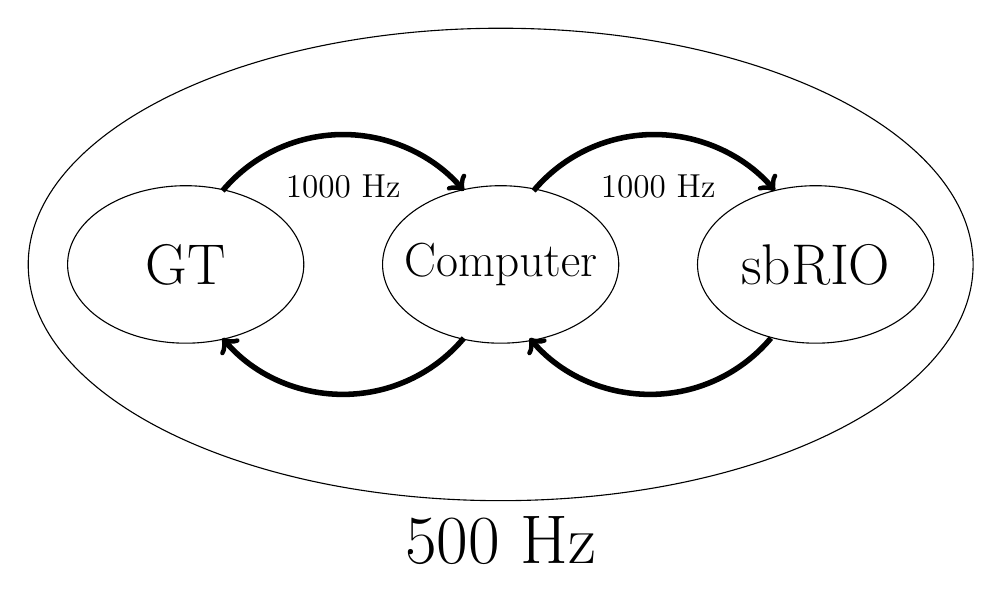
\begin{tikzpicture}

  \draw  (-3,0) ellipse (1.5 and 1)node (v1) {\LARGE Computer};
  \draw  (-7,0) ellipse (1.5 and 1)node{\huge GT};
  \draw  (1,0) ellipse (1.5 and 1)node{\huge sbRIO};


  \draw [->,line width=2pt](-6.5321,0.9356) arc (139.9997:40:2);
  \draw [<-,line width=2pt](-6.5321,-0.9356) arc (-139.9997:-40:2);
  \draw [<-,line width=2pt](-2.6321,-0.9356) arc (-139.9997:-40:2);
  \draw [->,line width=2pt](-2.5821,0.9356) arc (139.9997:40:2);


  \node at (-5,1) {\large 1000 Hz};
  \node at (-1,1) {\large 1000 Hz};
  \draw  (v1) ellipse (6 and 3);
  \node at (-3,-3.5) {\Huge 500 Hz};
  \end{tikzpicture}
  \end{figure}
\end{frame}

% the license
\begin{frame}<beamer>
\frametitle{Communication}


  \begin{itemize}
  \item<1-> Requirement for force feedback: 1000 Hz

  \item<2-> Maximum for the initial system: 100 Hz
  \item<3-> Our approach:
      \begin{itemize}
        \item<4-> Reducing the size of exchanged data
        \item<5-> Changing the transport protocol
      \end{itemize}
  \item<6-> Results: maximum of 638 Hz
  \end{itemize}


\end{frame}
% \begin{frame}<beamer>
% \frametitle{Friction model}
%   \begin{figure}[h]
% \centering
%   \begin{tikzpicture}
%   %axes
%   \draw [->,thick] (-3,0) -- (3,0);
%   \draw [->,thick] (0,-2.2) -- (0,2.2);
%   %model
%   \draw [ultra thick, color=blue] (0,-1.6) -- (0,1.6);
%   \draw [ultra thick, color=blue] (0,1.6) -- (3,1.6);
%   \draw [ultra thick, color=blue] (0,-1.6) -- (-3,-1.6);
%   %name of axis and variables
%   \node at (-0.4,1.6) {$\tau_s$};
%   \draw (-0.22,1.6) -- (-0.1,1.6);

%   \node at (3,0.4) {$\omega$};
%   \node at (0.4,2.2) {$\tau_f$};

%   \end{tikzpicture}
% \caption{final friction model}
% \label{fig:new_friction_model}
% \end{figure}
% \end{frame}
